\documentclass[conference]{IEEEtran}
\IEEEoverridecommandlockouts
% The preceding line is only needed to identify funding in the first footnote. If that is unneeded, please comment it out.
\usepackage{cite}
\usepackage{amsmath,amssymb,amsfonts}
\usepackage{algorithmic}
\usepackage{graphicx}
\usepackage{textcomp}
\usepackage{xcolor}
\def\BibTeX{{\rm B\kern-.05em{\sc i\kern-.025em b}\kern-.08em
    T\kern-.1667em\lower.7ex\hbox{E}\kern-.125emX}}
    
    
\graphicspath{ {./imgs/} }
    
\begin{document}

\title{Orange Detection Algorithm}

\author{\IEEEauthorblockN{Marshall Asch}
\IEEEauthorblockA{\textit{University of Guelph}\\
Guelph, Canada \\
masch@uoguelph.ca}
\and
\IEEEauthorblockN{Grant Douglas}
\IEEEauthorblockA{\textit{University of Guelph}\\
Guelph, Canada \\
gdouglas@uoguelph.ca}
}

\maketitle

\begin{abstract}
This document is a model and instructions for \LaTeX.
This and the IEEEtran.cls file define the components of your paper [title, text, heads, etc.]. *CRITICAL: Do Not Use Symbols, Special Characters, Footnotes, 
or Math in Paper Title or Abstract.
\end{abstract}

\begin{IEEEkeywords}
Image Processing, Fruit, Applied image colour segmentation, Automated counting
\end{IEEEkeywords}

\section{Introduction}

Counting and identifying the number of ripe fruits is important to automate harvesting fruits when they are ripe and to identify how many ripe fruits there are on a tree.

\section{Ease of Use}

\subsection{How we Selected the threshhold vales}


\section{Algorithms}




\subsection{Values} \label{values}


\begin{figure*}[htbp]
\centerline{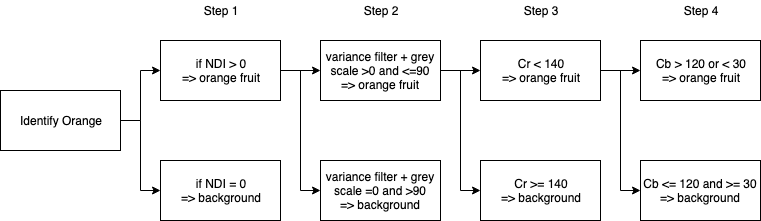
\includegraphics[width=\textwidth]{algo_stages}}
\caption{Outline of the proccess of the stages of the algorithm}
\label{fig}
\end{figure*}

\subsection{Stages}



\subsubsection{Step 1}
Run NDI 

\subsubsection{Step 2}
In the RGB colour space run a mean filter.

\subsubsection{Step 3}
convert the image to the YCrCb colour space.

run a threshold on the Cr values. how the threshold is discusses in sec. \ref{values}. 


\subsubsection{Step 4}

run a threshold on the Cb values. how the threshold is discusses in sec. \ref{values}. 



Then do a bit-wise and to create a mask

\begin{equation}
pixel_{final}=pixel_{NDI} \land pixel_{mean} \land pixel_{Cr} \land pixel_{Cb} 
\end{equation}

\subsubsection{Step 5}
Do a circle count  on the mask image


\begin{thebibliography}{00}
\bibitem{b1} G. Eason, B. Noble, and I. N. Sneddon, ``On certain integrals of Lipschitz-Hankel type involving products of Bessel functions,'' Phil. Trans. Roy. Soc. London, vol. A247, pp. 529--551, April 1955.
\bibitem{b2} J. Clerk Maxwell, A Treatise on Electricity and Magnetism, 3rd ed., vol. 2. Oxford: Clarendon, 1892, pp.68--73.
\bibitem{b3} I. S. Jacobs and C. P. Bean, ``Fine particles, thin films and exchange anisotropy,'' in Magnetism, vol. III, G. T. Rado and H. Suhl, Eds. New York: Academic, 1963, pp. 271--350.
\bibitem{b4} K. Elissa, ``Title of paper if known,'' unpublished.
\bibitem{b5} R. Nicole, ``Title of paper with only first word capitalized,'' J. Name Stand. Abbrev., in press.
\bibitem{b6} Y. Yorozu, M. Hirano, K. Oka, and Y. Tagawa, ``Electron spectroscopy studies on magneto-optical media and plastic substrate interface,'' IEEE Transl. J. Magn. Japan, vol. 2, pp. 740--741, August 1987 [Digests 9th Annual Conf. Magnetics Japan, p. 301, 1982].
\bibitem{b7} M. Young, The Technical Writer's Handbook. Mill Valley, CA: University Science, 1989.
\end{thebibliography}
\vspace{12pt}

\end{document}
